\section{Process' perspective}

\subsection{CI/CD Pipeline, Release, and Deployment}

This section describes how a change goes from development to a running production system. It starts in the repository, where new features, bug fixes and other updates are added through a shared Git workflow. From there, GitHub Actions handles the CI/CD pipeline.
\\
\\
Whenever code is pushed to the main branch or submitted through a pull request, the pipeline restores dependencies, builds the .NET solution, and runs automated tests. At the same time, static security checks are run to catch potential weaknesses.
\\
\\
When a version is ready, the pipeline also handles the release. Tagged versions produce builds for different operating systems, which makes it easy to connect a specific version of the code to the artifacts that were shipped. This improves traceability and makes it clear what has been delivered.
\\
\\
Deployment is the final step. The application runs in containers, and the infrastructure is defined using Terraform. Terraform provisions the required resources, such as the database and application instances. After that, Docker Compose is used to start and update the services. Because the entire environment is defined in code, deployments are consistent and repeatable rather than being performed manually, which reduces the risk of human error. As part of the deployment process, Trivy scans the Docker images for high and critical vulnerabilities. If it detects any such weaknesses, the scan fails and the deployment process is stopped before the images are pushed and the services are updated.
\\
\\
Below is a diagram showing the flow of our release-and-deploy workflow:

\begin{figure}[H]
    \centering
    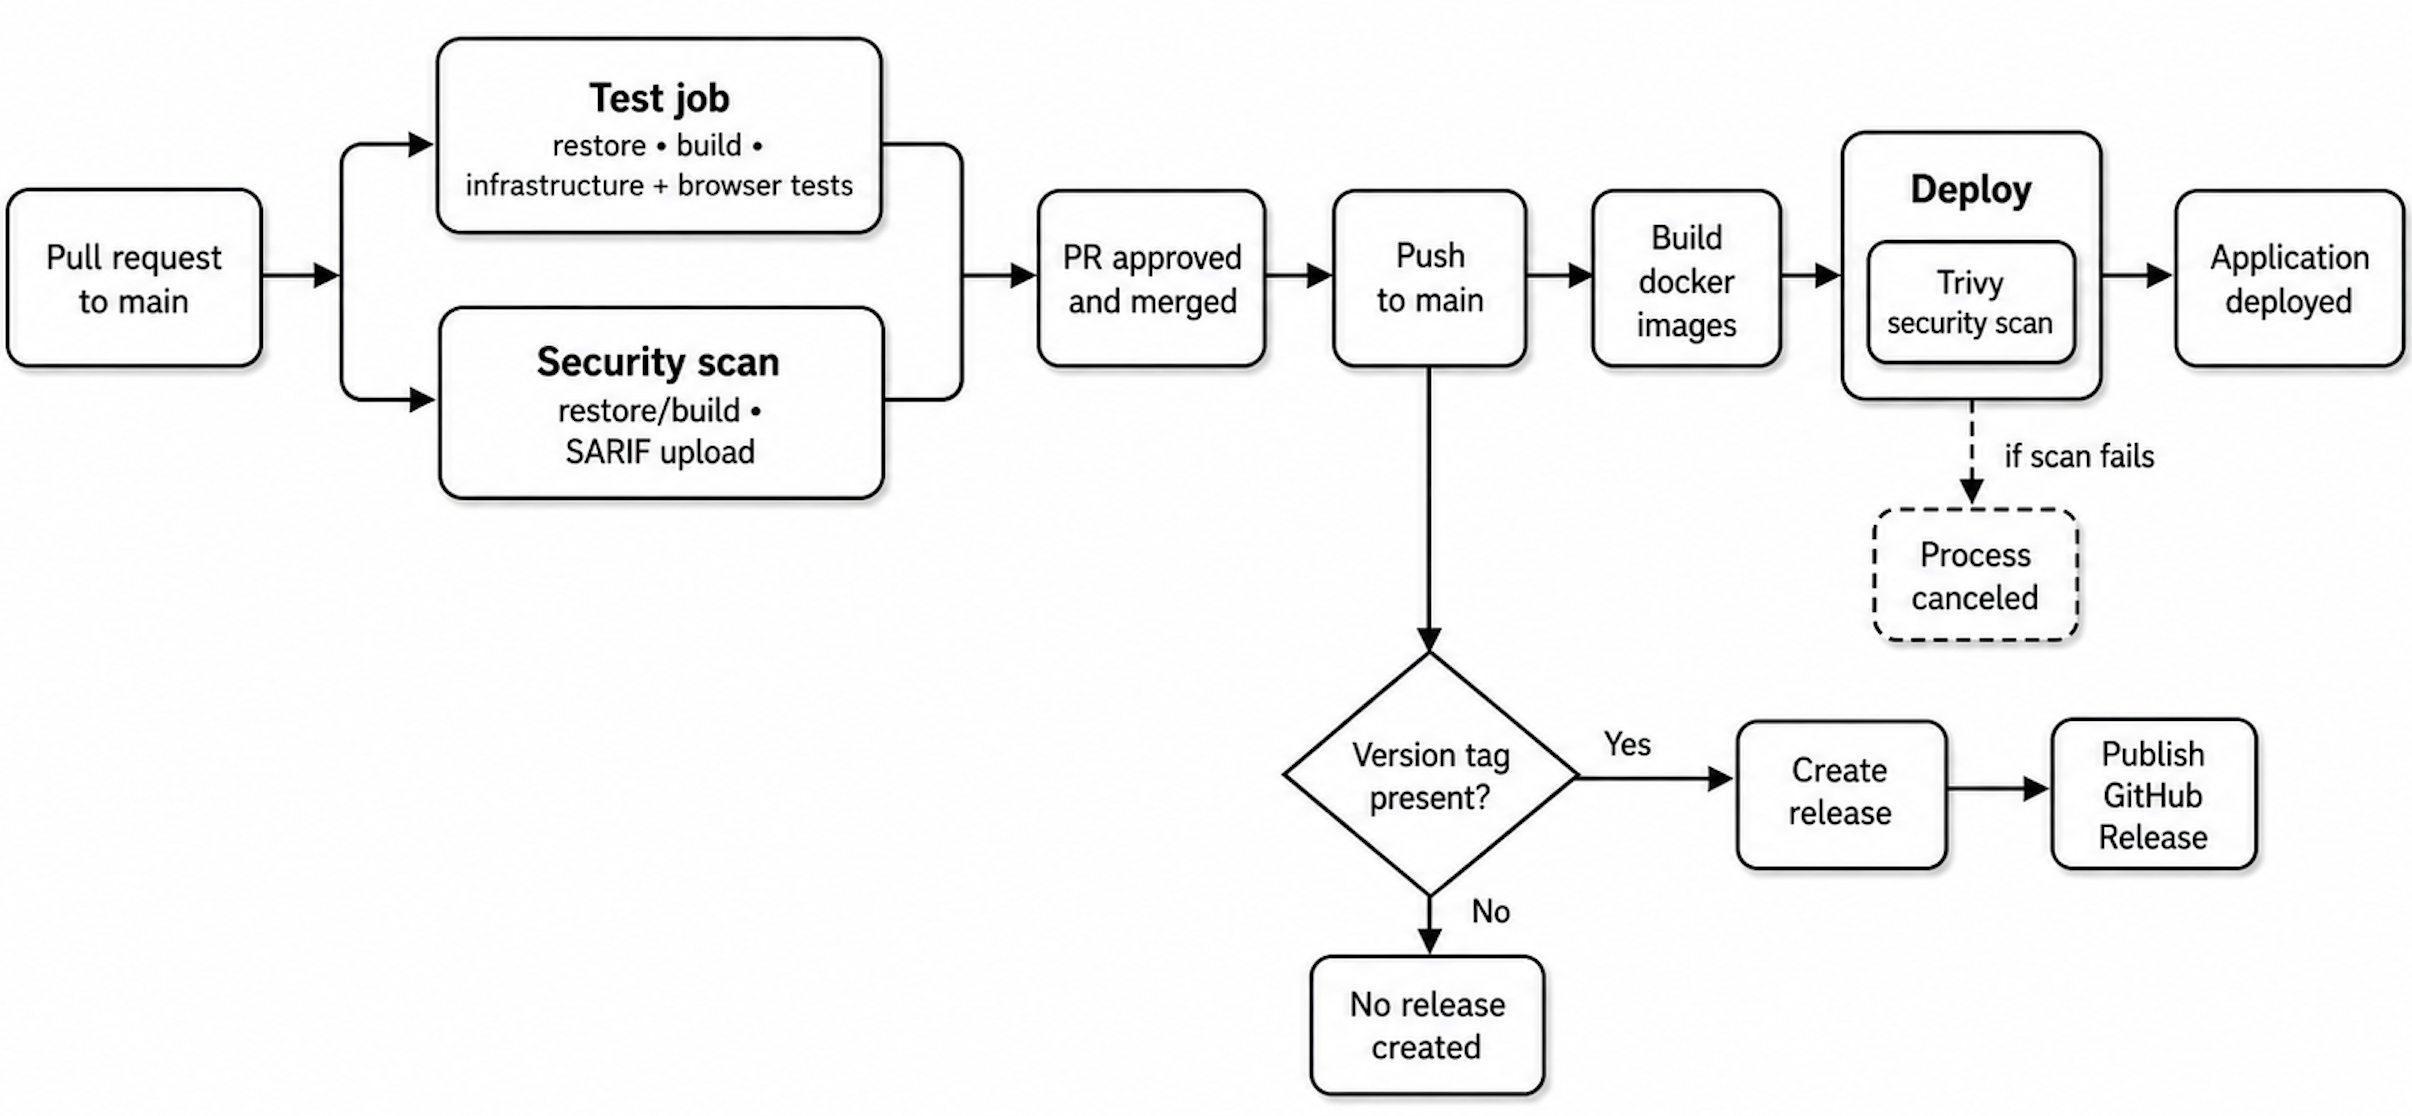
\includegraphics[width=\textwidth]{images/Release-Deploy.png}
    \caption{Release-and-deploy Workflow}
    \label{fig:Release-Deploy}
\end{figure}

\subsection{Monitoring}

Monitoring is based on Prometheus and Grafana. The web application and API expose metrics that Prometheus collects at regular intervals. This gives us a continuous view of how the system is behaving and helps detect issues like downtime or unusual traffic patterns. Grafana is used to display this data in dashboards, making it easier to visualize as well as understand what is going on.
\\
\\
\textbf{Our Monitoring Dashboards:}

\begin{figure}[H]
    \centering
    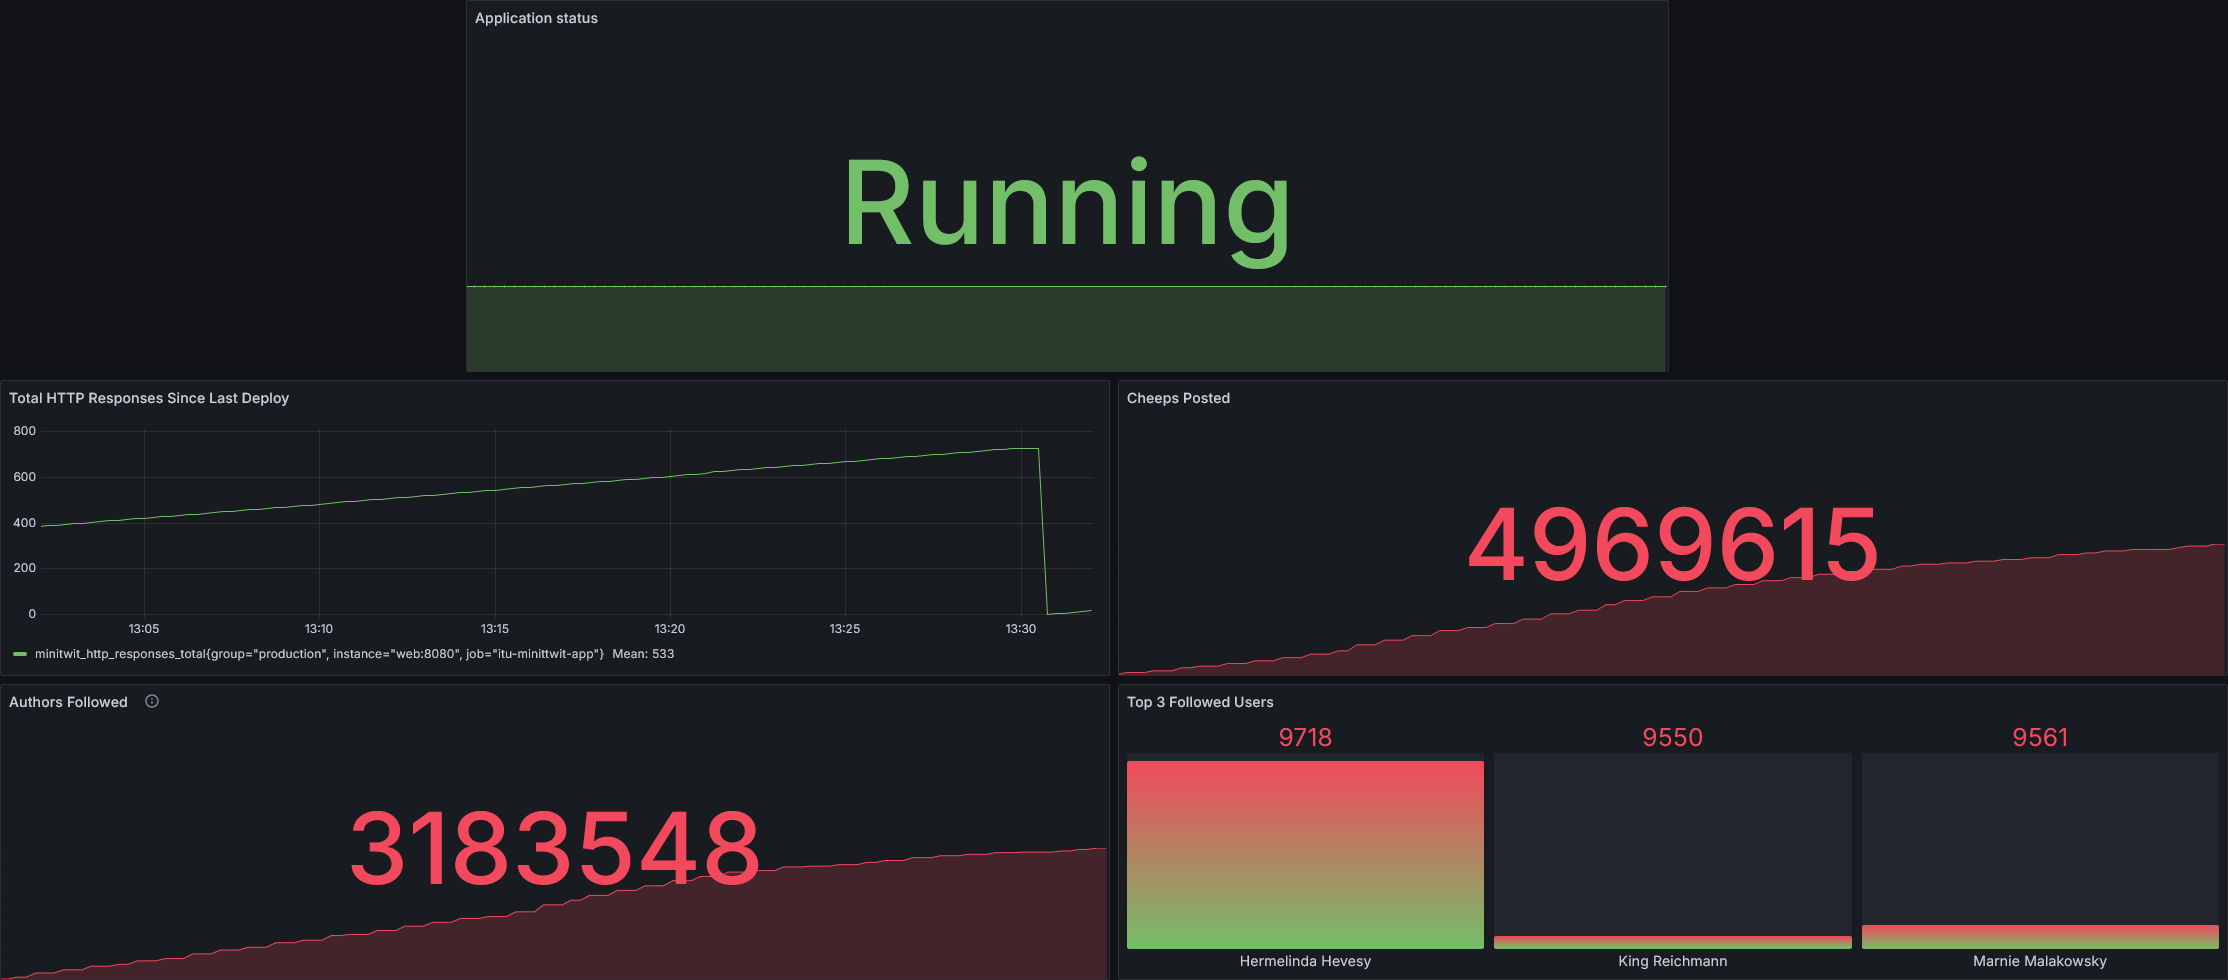
\includegraphics[width=0.8\textwidth]{images/Minitwit_Example_Dashboard.png}
    \caption{MiniTwit Example Dashboard}
    \label{fig:dashboard}
\end{figure}

\begin{figure}[H]
    \centering
    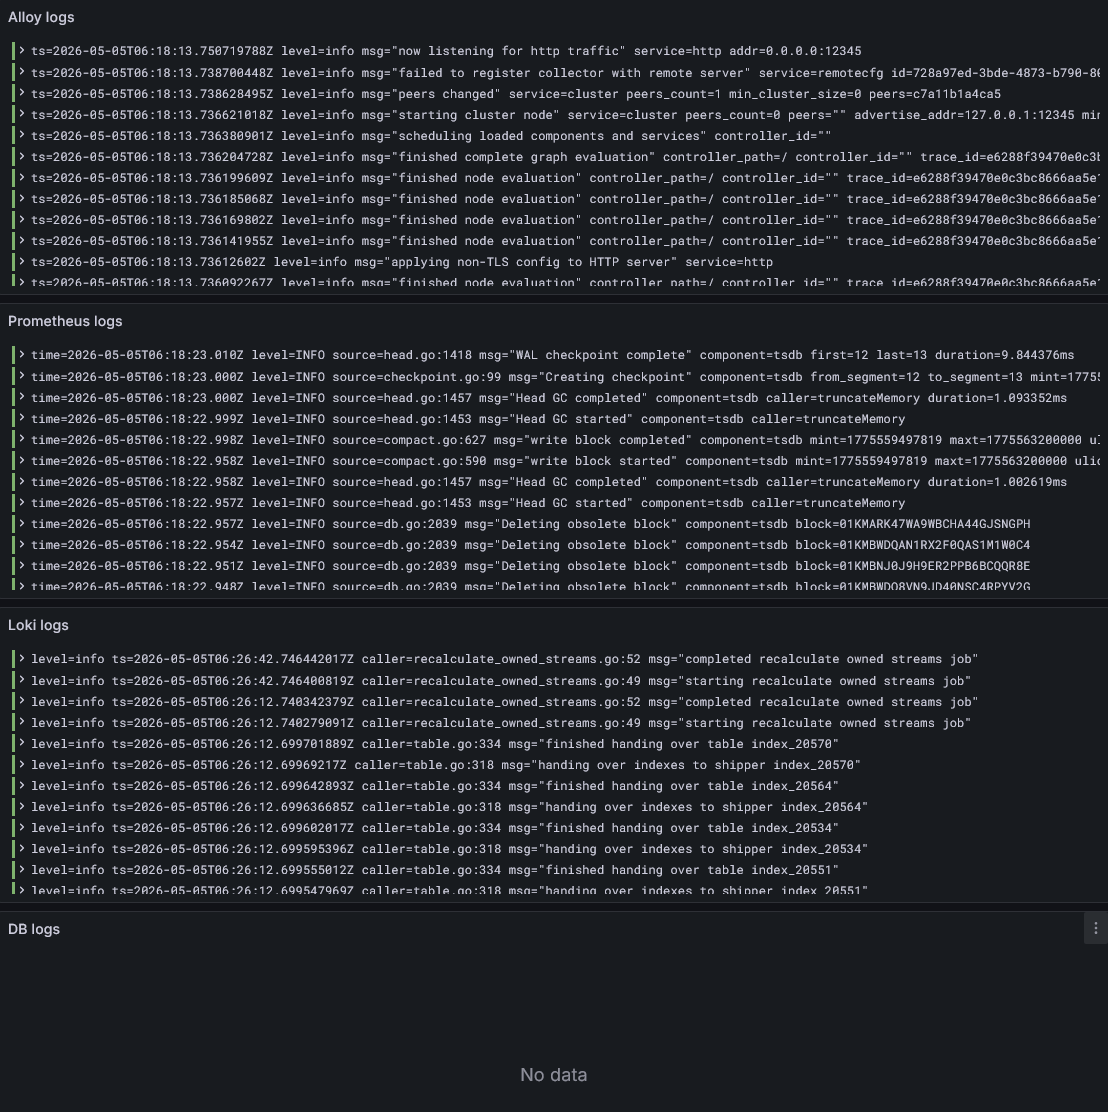
\includegraphics[width=0.7\textwidth]{images/Minitwit_Logging_Dashboard.png}
    \caption{MiniTwit Logging Dashboard}
    \label{fig:logging_dashboard}
\end{figure}

\subsection{Logging and Log Aggregation}

While monitoring shows overall trends, logging gives a more detailed picture of what is actually happening inside the system. Both the web application and the API writes logs to standard output in their containers. These logs include HTTP requests as well as important actions like registration, login, posting cheeps, and following other users.
\\
The logs are collected and brought together in one place. Docker handles them locally with rotation to avoid unlimited growth, and Alloy forwards them to Loki. Grafana is then used to visualize the logs. This makes it possible to investigate issues across the whole system instead of just a single machine. If something looks off in the metrics, the logs can be checked to find out why.

\subsection{Security Hardening} \label{sec: security}

Security is handled both in the pipeline and in the code. In the CI/CD process, static analysis tools, such as Trivy, help catch vulnerable code before being deployed. Container images are also scanned, and any issues are documented.
\\
In production, traffic is protected using TLS at the load balancers, and HTTPS is enforced outside of development. Sensitive data like connection strings is provided through environment variables instead of being stored in the codebase. Data-protection keys are stored in the database so authentication remains stable across restarts and multiple instances. Containers also run without root privileges, which limits the impact if something goes wrong. These steps don’t make the system fully secure, but they show that security has been taken into account throughout.

\subsection{Availability and Scaling}

Availability and scaling are handled through the infrastructure setup. Instead of running on a single server, the system uses two application instances behind two load balancers. Traffic is distributed using nginx and keepalived handles failover between load balancers. This means that if one component fails, another can take over.
\\
Containers are configured with restart policies and dependencies to improve reliability. The application can also scale by adding more instances using the same setup, which makes it easier to handle increased load without changing the overall design. The main limitation is the database, which is still a more centralized component. Even so, the combination of multiple instances, load balancing, and failover provides availability and future scaling.

